\chapter{Augmented Reality : Markerbased and location-based}

\section{Introduction}
For a few years, I have been a fan of Aframe and AR.js - these are fantastic tools for creating web-based Virtual and Augmented Reality.

\section{Marker-based}
Now AR.js has just got easier - no coding need with the Beta version of AR.js Studio \url{https://ar-js-org.github.io/studio/}

\begin{figure}
    \centering
    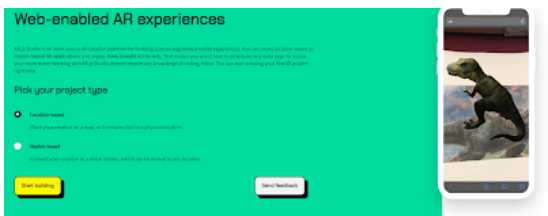
\includegraphics[width=10cm]{chapters/ChapterAR/webar1.png}
    \caption{AR.JS studio}
    \label{fig:arjsstudio}
\end{figure}

I am going to use the premade marker but you can upload your own, there is a guide to what makes a good marker. The premade marker you can download from the site using the download marker link underneath the marker. Apart from that, you don't have to do anything else to select the marker
\begin{figure}
    \centering
    
\includegraphics[width=5cm]{chapters/ChapterAR/webar6.png}
    \caption{marker}
    \label{fig:marker}
\end{figure}

Now you choose whether you want 3D object, image or video. So for this experiment, I going to use a free 3D model from https://sketchfab.com/3d-models/duck-6e039c6c606c4c26a1359514352629fd produced by likangning93 and released under a creative commons licence on Sketchfab. It is as simple as clicking upload file and browsing.

\begin{figure}
    \centering
    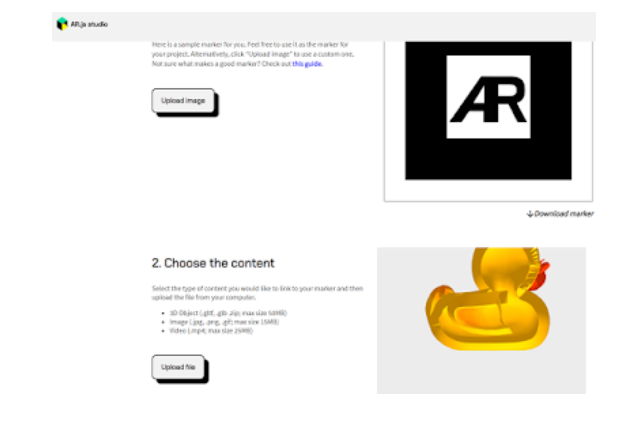
\includegraphics{chapters/ChapterAR/webar5.png}
    \caption{set up}
    \label{fig:my_setup}
\end{figure}

Last stage is exporting the project. Two options 
- Published to Github 
- Download package

My advice is, if you don't have your own web-server, get yourself a Github account and choose that option, and you just log-in to your account. You will need to give the project a name and then push Publish. Depending on your internet connection it can take a few seconds to a minute or so, but it is worth the wait.

So now you get back a \url{https://scottturneruon.github.io/Testobjectexs5y2/} 

Now just show the marker.
\begin{figure}
    \centering
    
\includegraphics[width=5cm]{chapters/ChapterAR/webar6.png}
    \caption{marker}
    \label{fig:marker}
\end{figure}

So to test I am typing this URL in a Safari browser (Chrome can play up) on my phone and allow access to my camera (see below or try it for yourself which is more fun).

\begin{figure}
    \centering
    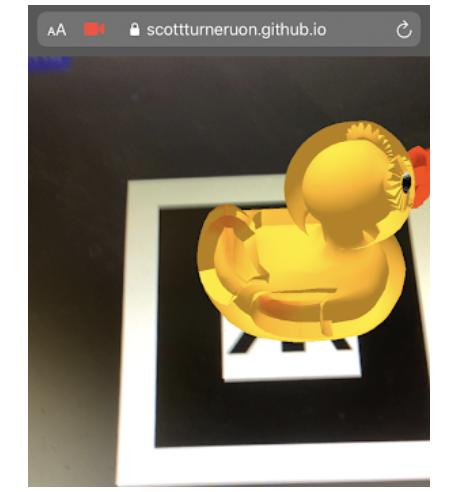
\includegraphics{chapters/ChapterAR/webar7.png}
    \caption{Floating duck}
    \label{fig:floatingduck}
\end{figure}

This Beta version is very good, no coding needed by the user and easy steps to an AR.  At the time of writing the only slight issue was you need to ensure that the file extensions were not capitalised but other than it is a great tool for produce a single AR example. I need to try the location-based version next.



\section{Location-based}
 Now AR.js has just got easier - no coding need with the Beta version of AR.js Studio  including using markers and the focus of this post, geo-located or markerless AR.
 
 It so easy I am going to show two examples. First going to the start screen of AR.js Studio https://ar-js-org.github.io/studio, select location based project type.
 
\begin{figure}
    \centering
    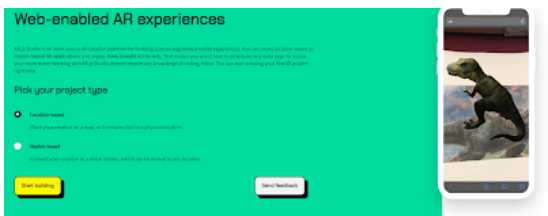
\includegraphics[width=10cm]{chapters/ChapterAR/webar1.png}
    \caption{AR.JS studio}
    \label{fig:arjsstudio}
\end{figure}
 
 You will then be asked for the longitude and latitude on where you want your AR to be located, up to 10 locations can be used - I have only used one to trial it. If you don't know these co-ordinates they have included a link to a site \url{https://www.latlong.net/}  that will give you these and you can then transfer them into AR.js Studio that is the geo location bit done. Now for the thing at the location.
 
 
So for the first experiment, I going to use a free 3D model from \url{https://sketchfab.com/3d-models/duck-6e039c6c606c4c26a1359514352629fd}  produced by likangning93 and released under a creative commons licence on Sketchfab. It is as simple as clicking upload file and browsing. The last stage is publishing it on GitHub and you getting a URL or downloading the files and which you can later add to a server - both really just a click option. 

So the Duck is shown below 

\begin{figure}
    \centering
    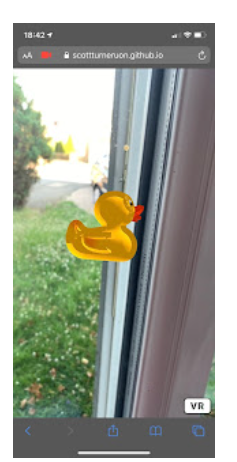
\includegraphics[width=10cm]{chapters/ChapterAR/webar3.png}
    \caption{Marker-less Duck}
    \label{fig:markerless_duck}
\end{figure}

So as a follow up and as I think Jupiter is such as a beautiful planet, I used a model by Miekle Roth on Sketchfab \url{https://sketchfab.com/3d-models/jupiter-c5275eb96af245e4a8453837ac728a62}  as a second geolocated object. 

So now I have Jupiter whenever I want - no I am not that power-mad.
 \begin{figure}
     \centering
     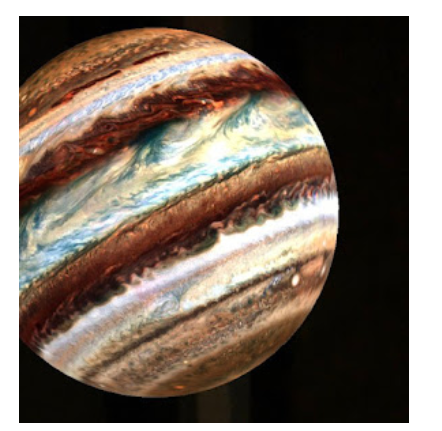
\includegraphics{chapters/ChapterAR/webar4.png}
     \caption{Jupiter}
     \label{fig:jupiter}
 \end{figure}
 
 Some interesting things I noticed it is relatively easy to do it, and I think the resources downloaded through AR.js Studio could be a great start on a more complex project. Initially, I didn't have location turned on my phone (obvious I know) but I could still see the object when I looked down - so that is great feature to have when you are trying out markerless AR to see what it could look like. 

Try AR.js Studio \url{https://ar-js-org.github.io/studio} for yourself.
